\documentclass[11pt,a4paper]{report}

\usepackage{polski}
\usepackage[utf8]{inputenc} 
\usepackage{a4wide}
\usepackage{tabularx}
\usepackage{lastpage}
\usepackage{fancyhdr}
\usepackage{graphicx}
\usepackage{caption}
\usepackage{latexsym}

% strona tytułowa
\begin{titlepage}
\title{\Huge Specyfikacja Funkcjonalna z Projektu\\\textsl{,,Tanks''}}
\author{Daniel Ślusarczyk i Jakub Łaba}
\date{28.04.2021}
\end {titlepage}

\renewcommand{\footrulewidth}{0pt}
\begin{document}
\maketitle

% zmiana numeracji sekcji 0.X -> X
\renewcommand*\thesection{\arabic{section}} 


% numeracja stron
\pagestyle{fancy}
\fancyhf{}
\rhead{\textsl{Sprecyfikacja Funkcjonalna "Tanks" | D. Ślusarczyk, J. Łaba}}
\rfoot{Strona \thepage \hspace{1pt} z \pageref{LastPage}}
\setcounter{page}{0}

% spis treści bez numeracji stron
\fancypagestyle{plain}
{
\fancyhead{} 
\fancyfoot{} 
}
\thispagestyle{empty} 
\tableofcontents 
\thispagestyle{empty}
\newpage

\fancypagestyle{plain} 
{
\fancyhead{} 
\fancyfoot[C]{\thepage}
}


% pierwsza sekcja
\section{Informacje ogólne}\label{sec:tekst}
\subsection {Przeznaczenie dokumentu}
Przeznaczeniem niniejszego dokumentu jest zawarcie szczegółów przedstawianego oprogramowania oraz omówienia zakresu prac, funkcjonalności produktu, a także interakcji zachodzących pomiędzy użytkownikiem a programem. Dokument ten pozwala na zapoznanie się z tematyką projektu i trudnościami z nim związanych. Ponadto jest niejako instrukcją obsługi pozwalającą na zgłębienie problemu prawidłowego i świadomego korzystania z oprogramowania. 

\subsection {Przeznaczenie programu}
Program służy do przeprowadzenia prostej gry opartej na rywalizacji dla dwóch graczy. Pozwala na indywidualne ustawienie konfiguracji przebiegu rozgrywki poprzez dobranie preferowanych parametrów. Niemniej jednak, oprogramowanie \textsl{,,Tanks''} jest dedykowane średnio-zaawansowanym informatycznie użytkownikom.

\subsection {Wymagania programu}
Program \textsl{,,Tanks''} jest wieloplatformowym oprogramowaniem przeznaczonym głównie dla systemu \textsl{,,Windows''}.  Prawidłowe działanie wymaga posiadania zainstalowanego środowiska uruchomieniowego Javy (JRE) służącego do uruchamiania aplikacji z rozszerzeniem \textsl{.jar}. Wszystkie potrzebne komponenty powinny zostać przygotowane przez dołączony instalator po przejściu przez proces instalacji.

\subsection {Problematyka -- wprowadzenie teoretyczne}
Gra jest dedykowana dwóm graczom rozmieszczonym po dwóch stronach okna rozgrywki, których zadaniem jest strzelanie do komórek w środkowej części za pomocą przypisanych czołgów. Gracze mają możliwość poruszania się swoimi jednostkami w górę i w dół, oraz obracania lufą czołgu +/- 60 stopni względem osi OX (prostej poziomej). Każdy pojazd strzela okrągłymi pociskami lecącymi z określoną prędkością, ograniczonych do pewnej ilości pocisków wystrzelonych jednocześnie. Dodatkowo na planszy może znajdować się tylko ograniczona ilość pocisków jednego gracza. Kwadratowe komórki, które są obiektem przyznawania punktów graczom dzielą się na trzy rodzaje: 
\begin {itemize}
\item\textbf {Zwykła komórka} --kwadratowy obiekt o wszystkich krawędziach wrażliwych na kontakt z pociskiem. Punkty za jej unicestwienie przyznawane są graczowi zadającemu końcowe obrażenia.
\item\textbf {Bomba} -- obiekt posiadający pancerne krawędzie z pominięciem górnej, która jest jedynym sposobem na zastrzelenie tej komórki. Dokonanie tego kończy grę.
\item\textbf {Kolonia} -- zbiór kwadratowych obiektów o wszystkich krawędziach wrażliwych na kontakt z pociskiem w losowej konfiguracji maksymalnie pięciu komórek. Gracz otrzymuję punkty o określonej wartości pomnożonej przez liczbę komórek należących do kolonii po zastrzeleniu ostatniej komórki w zbiorze. 
\end {itemize}
Wszystkie wyżej wymienione komórki poruszają się od górnej krawędzi okna rozgrywki do dolnej z określoną prędkością i mogą zostać zastrzelone tylko w momencie ich widoczności na polu bitwy. Ich aktualna wartość potrzebna do zastrzelenia znajduję się w centralnej części komórki.\\
Gra w sposób regularny zwiększa trudność rozgrywki poprzez zwiększanie wartości potrzebnej do unicestwienia komórki, szybkości komórek i wystrzeliwanych pocisków, oraz zmniejszanie promienia pocisku i długości boku komórki.
Koniec gry przewidują dwa scenariusze: upłynięcie określonego czasu rozgrywki lub zastrzelenie komórki bomby. Grę wygrywa gracz o większej ilości punktów w momencie zakończenia. 

\subsection {Cel Projektu}
Celem projektu „Tanks” jest stworzenie prostej gry z interfejsem graficznym w języku Java. Założeniami projektu są:
\begin {itemize}
\item Zawarcie w interfejsie gry liczby punktów obu graczy, okna komunikatów, licznika pozostałego czasu do zakończenia rozgrywki, liczby pocisków wystrzelonych przez graczy oraz okna z menu,
\item Zachowanie podejścia obiektowego w kodzie,
\item Zapisanie wyniku w formie pliku graficznego,
\item Przetestowanie kodu za pomocą automatycznych testów jednostkowych (JUnit),
\item Zachowanie wieloplatformowości oprogramowania.
\end {itemize}
\newpage

% druga sekcja
\section{Strona funkcjonalna programu}\label{sec:tekst}

\subsection {Uruchomienie programu}
Przy pierwszym uruchomieniu należy uruchomić instalator \textsl{,,InstallTanks.exe''} i postępować zgodnie z instrukcjami na ekranie. Instalator utworzy skrót aplikacji w wybranej przez użytkownika lokalizacji. Przy następnych uruchomieniach należy jedynie wybrać utworzony w wyniku instalacji skrót -- gra przed rozpoczęciem rozgrywki pozwala użytkownikowi na wprowadzenie własnych ustawień za pośrednictwem menu.

\subsection {Sterowanie}
\begin{tabularx}{\textwidth}{  X|Xl  }
 \hline
 \\Efekt                                   					& Przycisk\\
 \hline \hline
			\\Ruch czołgu w górę			&‘W’ dla gracza lewego, strzałka w górę dla gracza prawego\\
 \hline
			\\Ruch czołgu w dół				&‘S’ dla gracza lewego, strzałka w dół dla gracza prawego\\
 \hline
			\\Obrót lufy w górę				&‘A’ dla gracza lewego, strzałka w prawo dla gracza prawego\\
\hline
			\\Obrót lufy w dół				&‘D’ dla gracza lewego, strzałka w lewo dla gracza prawego\\
 \hline
			\\Oddanie strzału				&Spacja dla gracza lewego, prawy Shift dla gracza prawego\\
 \hline
			\\Pauza					&Escape\\
 \hline
\end{tabularx}

\subsection {Funkcjonalności programu}
Ekran ustawień, dostępny za pośrednictwem menu głównego, pozwala na dostosowywanie rozgrywki do potrzeb i wymagań użytkownika na wiele sposobów -- pozwala wybrać jeden z trzech predefiniowanych poziomów trudności, lub dostosować wszystkie parametry rozgrywki ręcznie.

\subsection {Wynik działania programu}
Po zakończeniu rozgrywki -- w wyniku upływu czasu przeznaczonego na rozgrywkę bądź w wyniku trafienia przez jednego z graczy komórki-bomby -- aplikacja wykona zrzut ekranu. Ponadto, wspomniane wyżej ustawienia gry będą umożliwiać zapisanie pożądanych parametrów rozgrywki w formie pliku konfiguracyjnego. W wyniku działania programu mogą powstać więc 2 rodzaje plików -- graficzne oraz konfiguracyjne.

\newpage
% trzecia sekcja
\section{Interfejs graficzny}

\subsection{Okno Menu}
Elementami obowiązkowymi okna menu są trzy przyciski: jeden odpowiedzialny za początek gry, drugi odpowiedzialny za przejście do ustawień, trzeci umożliwiający wyjście z gry. Na samej górze powinna znajdować się nazwa gry w sposób maksymalnie ostentacyjny. Poniższe dwa rysunki przedstawiają możliwe rozmieszczenie komponentów i proponowany styl dla tego okna.
\begin{figure}[!ht]
\centerline{\includegraphics{img/menu1.png}}
\caption{Szablon interfejsu okna menu}
\end{figure}
\newpage
\subsubsection{Wersja poglądowa}
\begin{figure}[!ht]
\centerline{\includegraphics{img/menu2.png}}
\caption{Wersja poglądowa okna menu}
\end{figure}
\newpage
\subsection{Okno Ustawień}
Elementami obowiązkowymi okna ustawień jest pole umożliwiające modyfikowanie parametrów domyślnych używanych tylko w przypadku problemów z plikiem konfiguracyjnym. Ważnymi aspektami tego okna są również pole umożliwiające podanie ścieżki do pliku konfiguracyjnego, \textsl{checkbox} z wyborem, czy po rozgrywce ma zostać wykonany zrzut ekranu i przycisk umożliwiający powrót do okna menu. Poniższe dwa rysunki przedstawiają możliwe rozmieszczenie komponentów i proponowany styl dla tego okna.
\begin{figure}[!ht]
\centerline{\includegraphics{img/sett1.png}}
\caption{Szablon interfejsu okna ustawień}
\end{figure}
\newpage
\subsubsection{Wersja poglądowa}
\begin{figure}[!ht]
\centerline{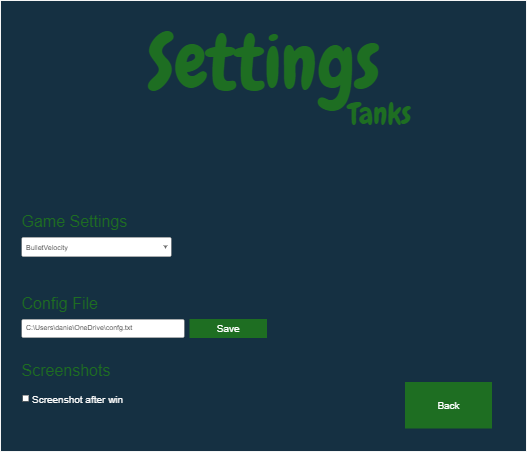
\includegraphics{img/sett2.png}}
\caption{Wersja poglądowa okna ustawień}
\end{figure}
\newpage
\subsection{Okno Gry}
Elementami obowiązkowymi okna gry są komponenty umożliwiające identyfikacje zwycięzcy wśród obu graczy (pola wyświetlające wynik). Dodatkowo \textsl{pole bitwy} powinno być widocznie odznaczone od reszty pól, a sam środek wypełniać licznik czasu do końca rozgrywki. Lewy i prawy skraj planszy jest przeznaczony na poruszanie się czołgów, a dolna krawędź \textsl{pola bitwy} na samym środku dla bomby. Pod nią znajduje się pole wyświetlające komunikaty. Poniższe dwa rysunki przedstawiają możliwe rozmieszczenie komponentów i proponowany styl dla tego okna.
\begin{figure}[!ht]
\centerline{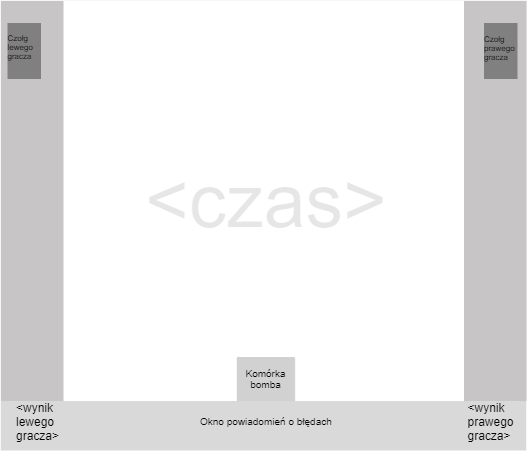
\includegraphics{img/game1.png}}
\caption{Szablon interfejsu okna rozgrywski}
\end{figure}
\newpage
\subsubsection{Wersja poglądowa}
\begin{figure}[!ht]
\centerline{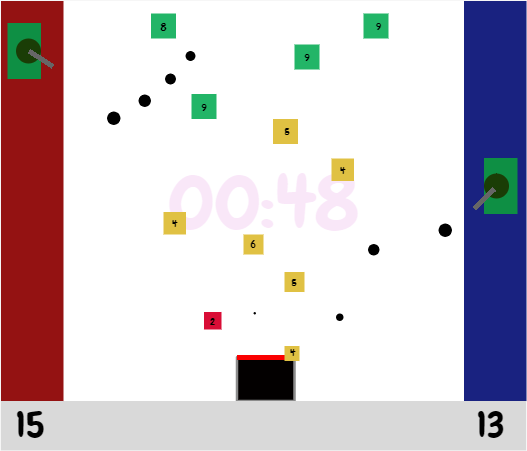
\includegraphics{img/game2.png}}
\caption{Wersja poglądowa okna rozgrywki}
\end{figure}
\newpage
%czwarta sekcja
\section{Parametry działania programu}
\subsection {Plik konfiguracyjny}
Plik konfiguracyjny jest zbiorem danych ustalającym szczegółowe zasady działania gry i pozwalającym na zastąpienie nimi wartości domyślnych przyjmowanych przez programu przy braku pliku konfiguracyjnego.

\subsection {Modyfikowalne parametry}
\begin{tabularx}{\linewidth}{  l|l|X  }
 \hline
 \\Indentyfikator                           &Nazwa			 &Opis\\
 \hline \hline
\\V1					& Bullet Velocity 		&Szybkość pocisków wystrzeliwanych przez graczy. Jednostka: [piksel/s] \\
 \hline
\\X1					&NumberOfBullets		&Maksymalna liczba pocisków gracza znajdująca się na planszy.\\
 \hline
\\V2					&CellVelocity			& Szybkość przemieszczania się komórki od górnej do dolnej krawędzi. Jednostka [piksel/s]\\
 \hline
\\H1 					&CellSize			& Długość boku kwadratu komórek. Jednostka: [piksel]\\
 \hline
\\P1 					&CellHealth 			&Wartość przypisana do każdej komórki symbolizująca liczbę kul potrzebną do unicestwienia mieszcząca się w przedziale od 1 do 9.  \\
 \hline
\\T2 					&CellRegenearationInterval	& Interwał czasowy pomiędzy kolejnymi wzrostami P1. Jednostka: [piksel]\\
 \hline
\\T1 					&Interval 			&Interwał czasowy pomiędzy kolejnymi przyrostami. Jednostka: [s]\\
 \hline
\\DV1 					&BulletVelocityIncrease 	&Przyrost szybkości wystrzeliwanego pocisku przez graczy dodawany co T1 sekund do V1. Jednostka: [piksel/s]\\
 \hline
\\DV2 					&CellVelocityIncrease 	&Przyrost szybkości poruszania się komórki dodawany co T1 sekund do V2. Jednostka: [piksel/s]\\
 \hline
\\DR1 					&BulletRadiusDecrease	&Spadek długości promienia wystrzeliwanego pocisku odejmowany co T1 sekund od R1. Jednostka: [piksel]\\
 \hline
\\DH1 					&CellSizeDecrease 		&Spadek długości boku kwadratu pojawiającej się komórki odejmowany co T1 sekund od H1. Jednostka: [piksel]\\
 \hline
\\T3 					&GameTime 			&Czas trwania rozgrywki. Jednostka: [s]\\
 \hline
\\IMG 					&ImageExtension 		&Format pliku graficznego tworzony przy zakończeniu gry. Jeśli nie jest podany żaden to plik nie jest tworzony.\\
 \hline
\end{tabularx}

\subsection {Struktura pliku konfiguracyjnego}
Przedstawiona poniżej stuktura pliku konfiguracyjnego przedstawia sposób prawidłowego przedstawienia elementów pliku. Miejsca ujęte w nawiasy trójkątne powinny zostać zastąpione oczekiwanymi wartościami zgodnie z wymaganiami przedstawionymi w nawiasach.\\
\textbf{Struktura:\\}
$<$Nazwa pliku konfiguracyjnego$>$\newline
[V1] BulletVelocity $<$liczba rzeczywista większa od 0$>$\newline
[X1] NumberOfBullets$<$liczba całkowita większa od 0$>$\newline
[R1] BulletRadius $<$liczba rzeczywista większa od 0$>$\newline
[V2] CellVelocity $<$liczba rzeczywista większa od 0$>$\newline
[H1] CellSize $<$liczba rzeczywista większa od 0$>$\newline
[P1] CellHealth $<$liczba całkowita większa od 0 i mniejsza od 9$>$\newline
[T2] CellRegenerationInterval $<$liczba rzeczywista większa od 0$>$\newline
[T1] Interval $<$liczba rzeczywista większa od 0$>$\newline
[DV1] BulletVelocityIncrease $<$liczba rzeczywista większa od 0$>$\newline
[DV2] CellVelocityIncrease $<$liczba rzeczywista większa od 0$>$\newline
[DR1] BulletRadiusDecrease$<$liczba rzeczywista większa od 0$>$\newline
[DH1] CellSizeDecrease $<$liczba rzeczywista większa od 0$>$\newline
[T3] GameTime $<$liczba całkowita większa od 0$>$\newline
[IMG] ImageExtension $<$PNG/ JPG /JPEG/ BMP$>$



\subsection {Przykładowy plik konfiguracyjny}

\begin{figure}[!ht]
\centerline{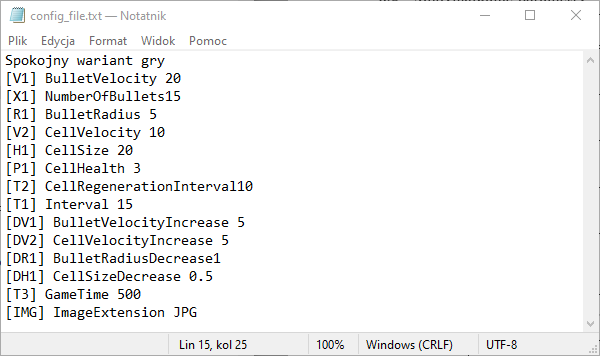
\includegraphics{img/config_example.png}}
\caption{Przykładowy plik konfiguracyjny}
\end{figure}

% piąta sekcja
\section{Przebieg działania programu}
\subsection {Scenariusz powszechny}
W domyślnym scenariuszu działania programu, użytkownik uruchamia rozgrywkę od razu lub najwpierw definiuje własne ustawienia zgodnie z instrukcją zawartą w podpunktach ,,Funkcjonalności programu'' oraz ,,Plik konfiguracyjny''. Następnie, po zakończeniu rozgrywki zostaje zapisany zrzut ekranu. Po przeprowadzeniu jednej gry można zamknąć aplikację, od razu uruchomić kolejną rozgrywkę z identycznymi ustawieniami lub powrócić do menu głównego w celu ich modyfikacji przed kolejną rozgrywką.

\subsection {Scenariusze ewentualne}
\subsubsection{Nieprawidłowy plik konfiguracyjny}
Program wczytuje cały plik konfiguracyjny linia po linii sprawdzając poprawność każdego wiersza pod kątem formatu. W przypadku znalezienia jakichkolwiek nieprawidłowości zostanie wyświetlony komunikat informujący użytkownika o nieprawnym pliku konfiguracyjnym z informacjami pozwalającymi na zdiagnozowanie problemu i zapytanie, czy kontynuować program z ustawieniami domyślnymi. Odpowiedź „Tak” pozwala na przeprowadzenie rozgrywki z ustawieniami domyślnymi. Odpowiedź „Nie” kończy działanie programu.
\subsubsection{Brak pliku konfiguracyjnego}
Program w przypadku braku pliku konfiguracyjnego wyświetla ostrzeżenie o braku pliku konfiguracyjnego, niezaburzające działania aplikacji. Dalszy przebieg programu odbywa się na podstawie domyślnych ustawień. 
\subsubsection{Nieprawidłowe działanie programu}
W działaniu aplikacji \textsl{,,Tanks''} mogą wystąpić błędy związane z nieprawidłowym przygotowaniem pliku konfiguracyjnego, poza tym nie przewiduje się żadnych błędów ponad standardowe wyjątki zgłaszane przez środowisko Javy.
\subsubsection{Komunikowanie błędów}


\begin {itemize}
\item\textbf {FILE\_INCOMPLETE [nazwa skrócona danej]} -- oznacza wybrakowanie informacji w pliku konfiguracyjnym (któregoś z parametrów brakuje). Przykładowy kod tego błędu: FILE\_INCOMPLETE [T3]-- oznacza, że w pliku brakuje informacji o czasie rozgrywki.
\item\textbf {INVALID\_DATA [nazwa skrócona danej]} -- oznacza wystąpienie nieprawidłowego typu lub wartości danej, odnoszącego się do podanego przez kod błędu parametru. Przykładowy kod tego błędu: INVALID\_DATA [DV1] -- oznacza, że w pliku wystąpił niewłaściwy typ parametru opisującego przyrost prędkości pocisków, tj. niebędący liczbą rzeczywistą bądź będący liczbą rzeczywistą wykraczającą poza dozwolony zakres.
\end {itemize}



\end{document}